\chapter{Testy systemu} \label{chapter_tests}

Jak zaznaczono w celu pracy (\ref{intro_objective}), prototyp systemu
ma być w pełni testowalny. Testy wykonywane są wewnątrz potoku ciągłej integracji 
(\textit{CI/CD}), opisanym w rozdziale \ref{chapter_deployment}. Niniejszy rozdział opisuje
rozwiązania zastosowane w celu przetestowania działania systemu.
Wykonane w projekcie testy dzielą się na cztery kategorie:

\begin{itemize}
    \item jednostkowe,
    \item integracyjne,
    \item systemowe,
    \item terenowe.
\end{itemize}

\noindent
\textit{Uwaga:} w pracy opisane są tylko testy, które zostały
napisane napisane przez autora. Obejmuje to testy jednostkowe systemu telemetrii,
testy integracyjne skonteneryzowanego symulatora drona oraz testy systemowe.

\section{Testy jednostkowe}

Testy jednostkowe obejmują sprawdzanie poprawności zachowania implementacji 
konkretnego komponentu, za pomocą zdefiniowanych przez programistę
przypadków testowych. Testy tego typu nie wykorzystują zewnętrznych 
interfejsów komponentu takich jak gniazda sieciowe czy urządzenia peryferyjne --
operują jedynie na warstwie logicznej komponentu, sprawdzając zachowanie 
abstrakcji programistycznej.
Tabela \ref{telem_server_unit_tests} zawiera 
opis testów jednostkowych sprawdzających działanie serwera
obsługującego telemetrię.

\begin{table}[H]
	\centering\small
	\caption{
        Testy jednostkowe serwera obsługującego telemetrię.
	}
	\label{telem_server_unit_tests}
    
    \begin{tabularx}{\textwidth} { 
        | >{\raggedright\arraybackslash}X 
        | >{\raggedright\arraybackslash}X | }
        \hline
        \textbf{Nazwa testu} & \textbf{Opis testu} \\
        \hline
        \texttt{test\_init\_state} & Sprawdzenie stanu początkowego obiektu reprezentującego serwer telemetrii. \\
        \hline
        \texttt{test\_adding\_new\_flight} & Sprawdzenie czy nadejście pakietu telemetrii spowoduje zarejestrowanie nowego aktywnego lotu. \\
        \hline
        \texttt{test\_new\_packet\_from\_existing\_flight  } & Sprawdzenie czy nadejście pakietu telemetrii z lotu o takim samym identyfikatorze co poprzednio otrzymany pakiet, spowoduje dopisanie pakietu do już istniejącego aktywnego lotu (nie zaś stworzenie nowego aktywnego lotu).\\
        \hline
        \texttt{test\_adding\_two\_flights} & Sprawdzenie czy utrzymanie pakietów o dwóch różnych identyfikatorach lotu spowoduje utworzenie dwóch aktywnych lotów. \\
        \hline
        \texttt{test\_flight\_archivisation\_on\_timeout} & Sprawdzenie czy po upłynięciu 20 sekund od otrzymania ostatniego pakietu, lot zostanie uznany za zakończony i przesłany do archiwizacji. \\
        \hline
        \texttt{test\_behaviour\_when} \texttt{getting\_invalid\_packet\_type} & Sprawdzenie czy w przypadku otrzymania pakietu o niewłaściwym typie zostanie zgłoszony wyjątek. \\
        \hline
     \end{tabularx}
\end{table}

\subsection{Testy jednostkowe w potoku \textit{CI/CD}}
Wykonywanie testów w potoku \textit{CI/CD} zwiększa sprawność
pracy z systemami kontroli wersji. W przypadku implementowania nowej 
funkcji na gałęzi (\textit{branch}), potok \textit{CI/CD} pozwala określić,
czy nowa funkcjonalność nie destabilizuje systemu -- ostrzegając przed 
przyjęciem na główną gałąź (\textit{master branch}) kodu, który nie przeszedł
testów jednostkowych. Rysunek \ref{failed_pipeline} przedstawia przykład
takiego zachowania w usłudze \textit{GitLab}.

\begin{figure}[H]
	\centering
	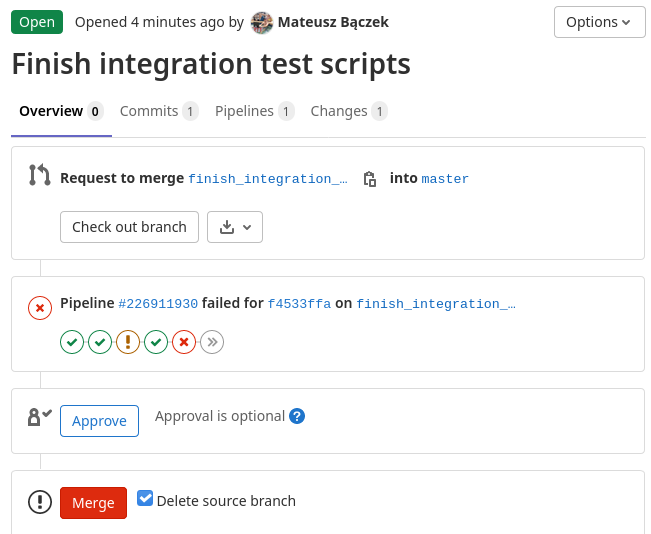
\includegraphics[width=0.8\linewidth]{rys05/failed_pipeline.png}
    \caption{
        Widok interfejsu scalania gałęzi w serwisie \textit{GitLab}.
        Gałąź \texttt{finish\_integration\_tests} nie przechodzi testów
        w potoku \textit{CI/CD}. Administrator repozytorium natychmiast
        otrzymuje informację, że kod nie jest jeszcze gotowy do scalenia.
    }
	\label{failed_pipeline}
\end{figure}

\section{Testy systemowe}

Realizowany w pracy system nie ogranicza się do pojedynczego,
samodzielnego komponentu, zawiera kilka równolegle działających
usług. testy jednostkowe nie są w takim przypadku wystarczające,
aby gruntownie sprawdzić poprawność działania kodu. 

Dodatkowym wyzwaniem przy projektowaniu testów jest interakcja z dronem,
którego kontroler lotu komunikuje się z systemem za pośrednictwem 
interfejsu \texttt{UART}, podłączonego do komputera pokładowego.
Błąd w komunikacji z kontrolerem lotu może doprowadzić do 
rozbicia maszyny, straty są tutaj zupełnie realne, inaczej
niż w przypadku testowania systemów pracujących jedynie na serwerach. 

\subsection{
    Symulacja i symulatory
    % \color{white}\cite{simulation_and_simulacra}
}

Symulatory lotu są szeroko wykorzystywane w przemyśle lotniczym
\cite{simulation_and_simulators}. Amatorskie otwartoźródłowe kontrolery
lotu nie są tutaj wyjątkiem -- jak wspomniano~w rozdziale poświęconym
kontrolerom lotu (\ref{flight_controller}), wykorzystywane w projekcie 
oprogramowanie \textit{ArduPilot} ma możliwość pracy w trybie \textit{SITL}
(\textit{software in the loop}). Jest to możliwe dzięki specjalnym opcjom,
które można ustawić w trakcie kompilacji. Opcje umożliwiają przemapowanie
interfejsów kontrolujących peryferia samolotu na ich wirtualne odpowiedniki,
które podłączane są do symulatora. Kod sterujący zachowaniem drona 
oraz dane telemetryczne pozostają takie same jak w przypadku
pracy na prawdziwej maszynie. Szczegółowy diagram 
ilustrujący przemapowywane peryferia kontrolera lotu 
zawarty jest na rysunku~\ref{sitl_diagram}.

\begin{figure}[H]
	\centering
	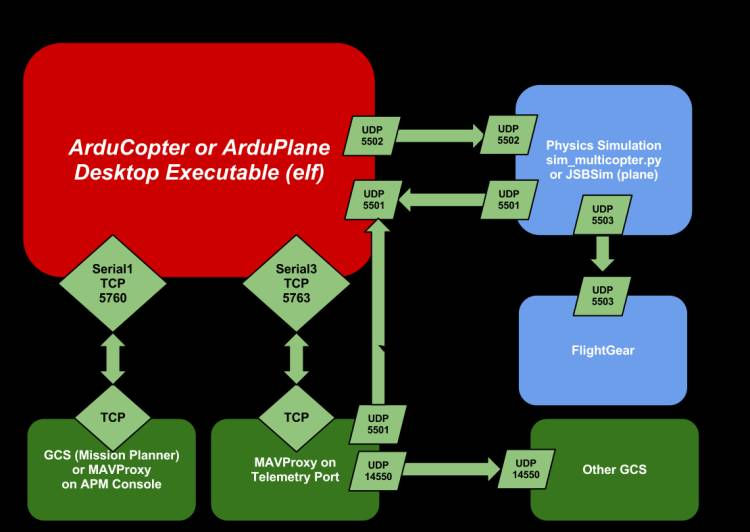
\includegraphics[width=0.9\linewidth]{rys05/sitl.jpg}
    \caption{
        Diagram zaczerpięty z dokumentacji \textit{ArduPilota}
        \cite{ardupilot_sitl}, ilustrujący działanie symulatora SITL.
    }
	\label{sitl_diagram}
\end{figure}


Ponieważ jedyna zmiana w wynikowym pliku wykonywalnym
z kontrolerem lotu to przemapowane interfejsy peryferiów,
komunikacja z kontrolerem lotu nadal działa w dokładnie
taki sam sposób. Kod, który był w stanie skomunikować
się z kontrolerem lotu działającym w trybie \textit{SITL},
będzie na pewno działał również na prawdziwej maszynie
(wyjątkiem byłaby oczywiście usterka sprzętowa, jednak takie
problemy leżą poza zakresem odpowiedzialności kodu).

Listing \ref{list:connecting_to_ardupilot_or_sitl} ilustruje,
jak zależnie od parametru konfiguracyjnego, skrypt sterujący 
dronem będzie próbował podłączyć się do prawdziwej maszyny lub
do symulatora. Jedyną różnicą są parametry w konstruktorze
obiektu połączenia, pozostały kod nie musi być modyfikowany
gdy przechodzi się z symulatora na prawdziwego drona.

\begin{lstlisting}[
    language=Python,
    label=list:connecting_to_ardupilot_or_sitl,
    caption={
        Przykład kodu łączącego się z prawdziwym dronem lub 
        z symulatorem lotu, zależnie od wartości parametru
        \texttt{USE\_SITL}. Utworzony obiekt \texttt{connection},
        reprezentujący połączenie, zawsze zachowuje się w taki
        sam sposób, niezależnie czy wykorzystywana jest
        prawdziwa maszyna czy symulator. 
    },
    basicstyle=\footnotesize\ttfamily
]
if USE_SITL:
    connection = mavutil.mavlink_connection(
        'udpin:0.0.0.0:14551' # Połączenie z symulatorem na porcie UDP
    )

else:    
    connection = mavutil.mavlink_connection(
        '/dev/ttyS0', # Połączenie z dronem za pomocą interfejsu UART
        baud=57600
    )
# Dalszy kod wykorzystujący obiekt `connection`.
# Nie ma znaczenia czy `connection` oznacza połączenie
# do symulatora czy do prawdziwego drona/samolotu
\end{lstlisting}

\subsection{\textit{SITL} i automatyczne testy w potoku \textit{CI/CD}}

Jak opisano w rozdziale \ref{chapter_deployment}, wszystkie komponenty systemu
docelowo uruchamiane są w kontenerach. Takie rozwiązanie pozwala na zagwarantowanie
poprawnego wdrożenia systemu na serwerze produkcyjnym. Równocześnie, kontenery wysyłane
na serwer produkcyjny można wcześniej przetestować w wirtualnym środowisku testowym.

Na potrzeby projektu, symulator kontrolera lotu został zkonteneryzowany i wykorzystany
w potoku \textit{CI/CD} do testów systemowych, angażujących wszystkie komponenty systemu.
Zespół pracujący nad projektem używał gotowego kontenera z symulatorem,
aby przeprowadzać testy na własnych maszynach. Takie rozwiązanie eliminuje wszystkie
problemy, jakie mogą pojawić się podczas wykorzystywania oprogramowania którego
konfiguracja jest bardzo złożona -- tak jak w przypadku symulatora lotu.

\subsection{Budowanie testów systemowych z wykorzystaniem \textit{Gitlab CI}}

Do uruchamiania testów systemowych przeznaczony został dedytkowany serwer
Linux. Serwer służył za platformę, na której uruchamiane były wszystkie 
komponenty systemu. Diagram \ref{system_tests_diagram} ilustruje 
sposób wykorzystywania dedykowanego serwera w celu przeprowadzenia 
testów ystemowych

\begin{figure}[H]
	\centering
	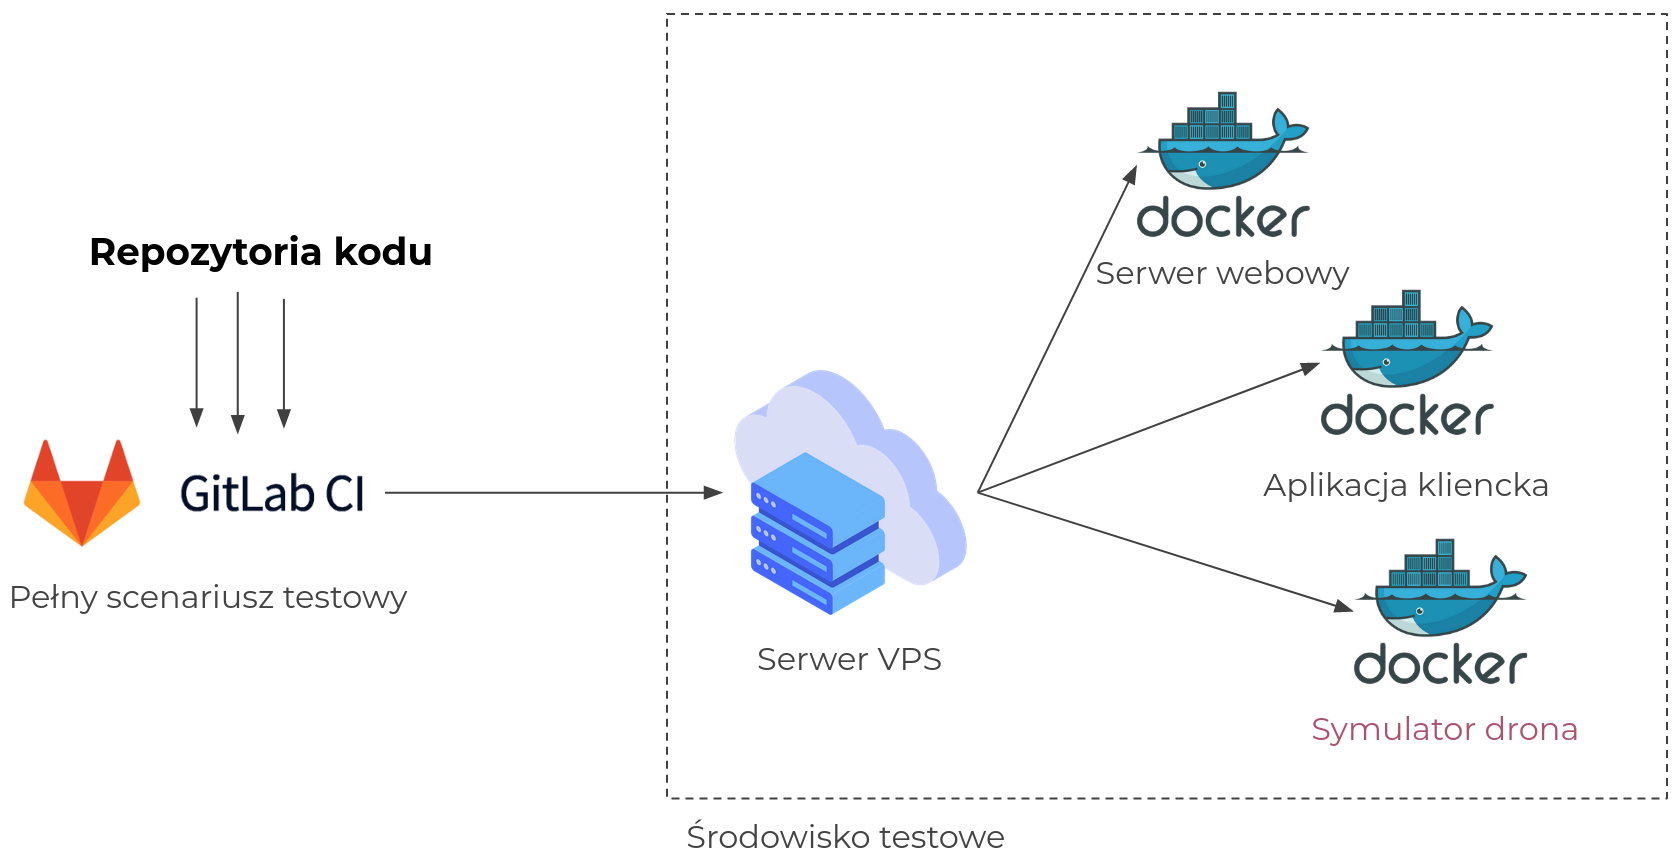
\includegraphics[width=\linewidth]{rys05/integration_tests_diagram.png}
    \caption{
        Pełne testy systemowe na dedykowanym serwerze.
    }
	\label{system_tests_diagram}
\end{figure}

\subsection{Konfiguracja serwera zarządzanego przez \textit{Gitlab CI}}

Platforma \textit{GitLab} umożliwia uruchamianie testów na własnej
infrastrukturze, w ramach usług dostępnych dla darmowych kont.
Infrastruktura platformy domyślnie pozwala jedynie
na testowanie wewnątrz izolowanych kontenerów \texttt{docker}.
Jest to rozwiązanie zupełnie wystarczające w przypadku testów jednostkowych.
Uruchomienie pełnego systemu w sztucznym środowisku wymaga jednak
większej kontroli nad serwerem testowym. \textit{Gitlab CI} pozwala
na podłączenie własnych serwerów do swojej sieci -- dzięki takiemu rozwiązaniu
użytkownicy mogą wykorzystywać pełne możliwości potoków ciągłej integracji.

Podłączony do systemu serwer wykonuje skrypty uruchamiające testy systemowe 
bezpośrednio na serwerze, co pozwala na równoległe uruchomienie wielu kontenerów 
\texttt{docker} oraz monitorowanie ich pracy z zewnątrz -- jak pokazano
na diagramie \ref{system_tests_diagram}.

\subsection{Definiowanie wieloetapowych testów systemowych}

W ramach testów systemowych testowane są wpierw pojedyncze kontenery --
nie są to jednak testy jednostkowe. Uruchamiany jest cały kontener zawierający
komponent systemu, następnie jest on testowany przez \textbf{zewnętrzny} skrypt.
W przypadku aplikacji klienckiej, uruchamiana jest sterowana automatycznie 
przeglądarka internetowa, która symuluje zachowanie prawdziwego użytkownika,
tworząc nową trasę przelotu drona. W przypadku serwera \textit{REST API}, wykonywane
są zapytania \textit{http} weryfikujące poprawność działania \textit{API}.

Po przetestowaniu pojedynych kontenerów, uruchamiane są testy angażujące
wiele kontenerów -- sprawdzające czy komponenty systemu będą ze sobą współpracowały.
Przykładowy scenariusz testowy zawiera:

\begin{enumerate}
    \item Uruchomienie kontenerów:
    \begin{itemize}
        \item symulatora kontrolera lotu,
        \item aplikacji sterującej dronem,
        \item aplikacji klienckiej
        \item serwera telemetrii
        \item serwera API.
    \end{itemize}
    \item Wykorzystanie zdalnie sterowanej przeglądarki w
            celu dodania nowej trasy przelotu w aplikacji klienckiej.
    \item Sprawdzenie, czy w aplikacji klienckiej pojawi się telemetria z drona,
            wykonującego zaplanowaną trasę.
\end{enumerate}

Taki test angażuje wszystkie uruchamiane komponenty. Skrypt wykonujący test
musi jedynie sterować aplikacją kliencką i weryfikować, czy pojawiają się
w niej dane pochodzące z pozostałych komponentów systemu.

\subsubsection{Etapy testów w \textit{GitLab CI}}

Platforma \textit{GitLab CI} pozwala na podzielenie testów na etapy. 
Każdy etap składa się z określonej liczby zadań. Aby potok \textit{CI/CD}
mógł przejść do kolejnego etapu, muszą zostać wykonane wszystkie zadania 
z poprzednich etapów. W przypadku testów systemowych oznacza to, że wpierw
zweryfikowane musi zostać działanie wszystkich kontenerów składających się
na system, następnie testowane są interakcje między komponentami. 
Finalny zestaw testów systemowych (\textit{test pipeline}), które były
wykonywane na systemie ilustruje rysunek \ref{pipeline_gitlab_ci}.\\
\\
\noindent
\textit{Uwaga:} etapy takie jak \textit{Pull images} czy \textit{Clean after component tests}
sprawdzają stan serwera przed i po wykonaniu etapu testów. Jest to wymagane, ponieważ testy
nie ograniczają się do izolowanych kontenerów dockera, lecz wymagaja komunikowania się
z komponentami za pomocą skryptów uruchamianych bezpośrednio na serwerze testowym. 
Etapy wykonywane pomiędzy testami weryfikują, czy konkretny etap testów zakończył 
się w odpowiedni sposób; nie pozostawił na serwerze działających procesów lub kontenerów.

\begin{figure}[H]
	\centering
	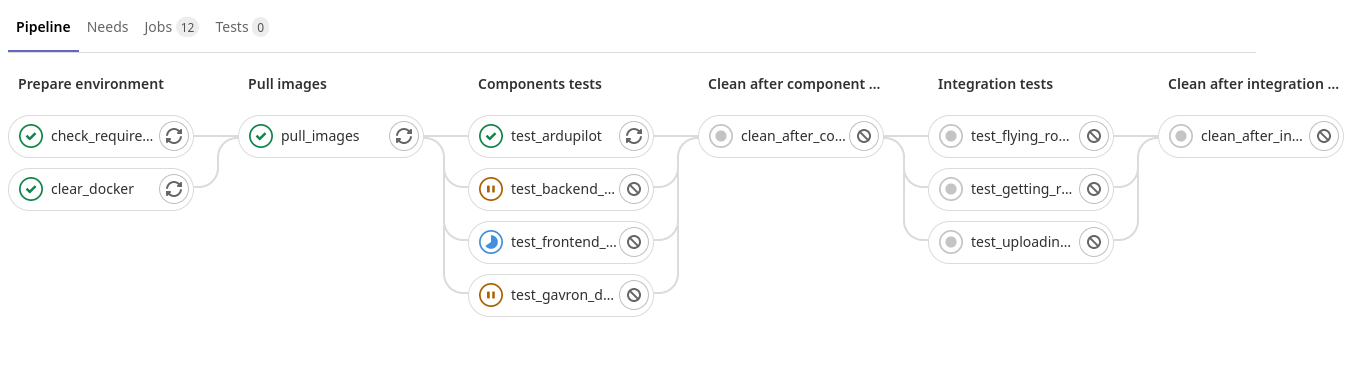
\includegraphics[width=\linewidth]{rys05/pipeline.png}
    \caption{
        Interfejs \textit{GitLab CI} prezentujący postęp w wykonywaniu
        wieloetapowych testów systemowych.
    }
	\label{pipeline_gitlab_ci}
\end{figure}

\section{Testy w terenie}

\subsection{Wczesne etapy rozwoju systemu} \label{early_tests}

Ze względu na pandemię COVID-19, system testowany był w terenie jedynie trzy razy.
Podczas pierwszych testów, dron z kamerą nie był jeszcze przygotowany, system został więc 
zaadaptowany do wykorzystania w jednym z samolotów Akademickiego Klubu Lotniczego (\ref{test_sae}).
Testom została poddana aplikacja kliencka i system obsługi telemetrii.

\begin{figure}[H]
	\centering
	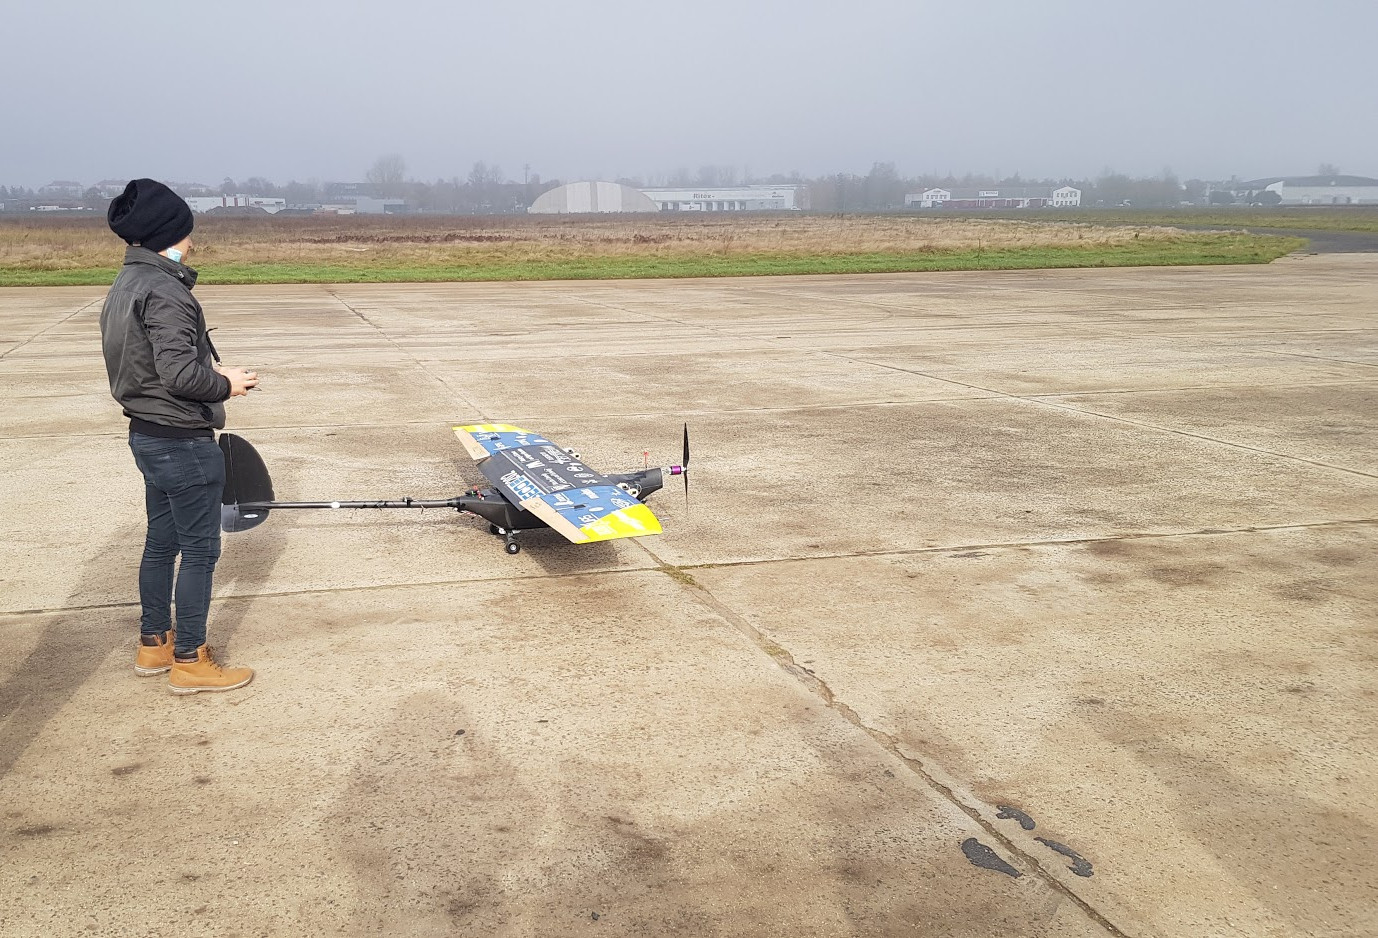
\includegraphics[width=0.8\linewidth]{rys05/test_sae.jpg}
    \caption{
        Pierwsze loty testowe, wykorzystujące jeden z samolotów Akademickiego
        Klubu Lotniczego. Testy objęły aplikację kliencką i system obsługi telemetrii.
    }
	\label{test_sae}
\end{figure}

\begin{figure}[H]
	\centering
	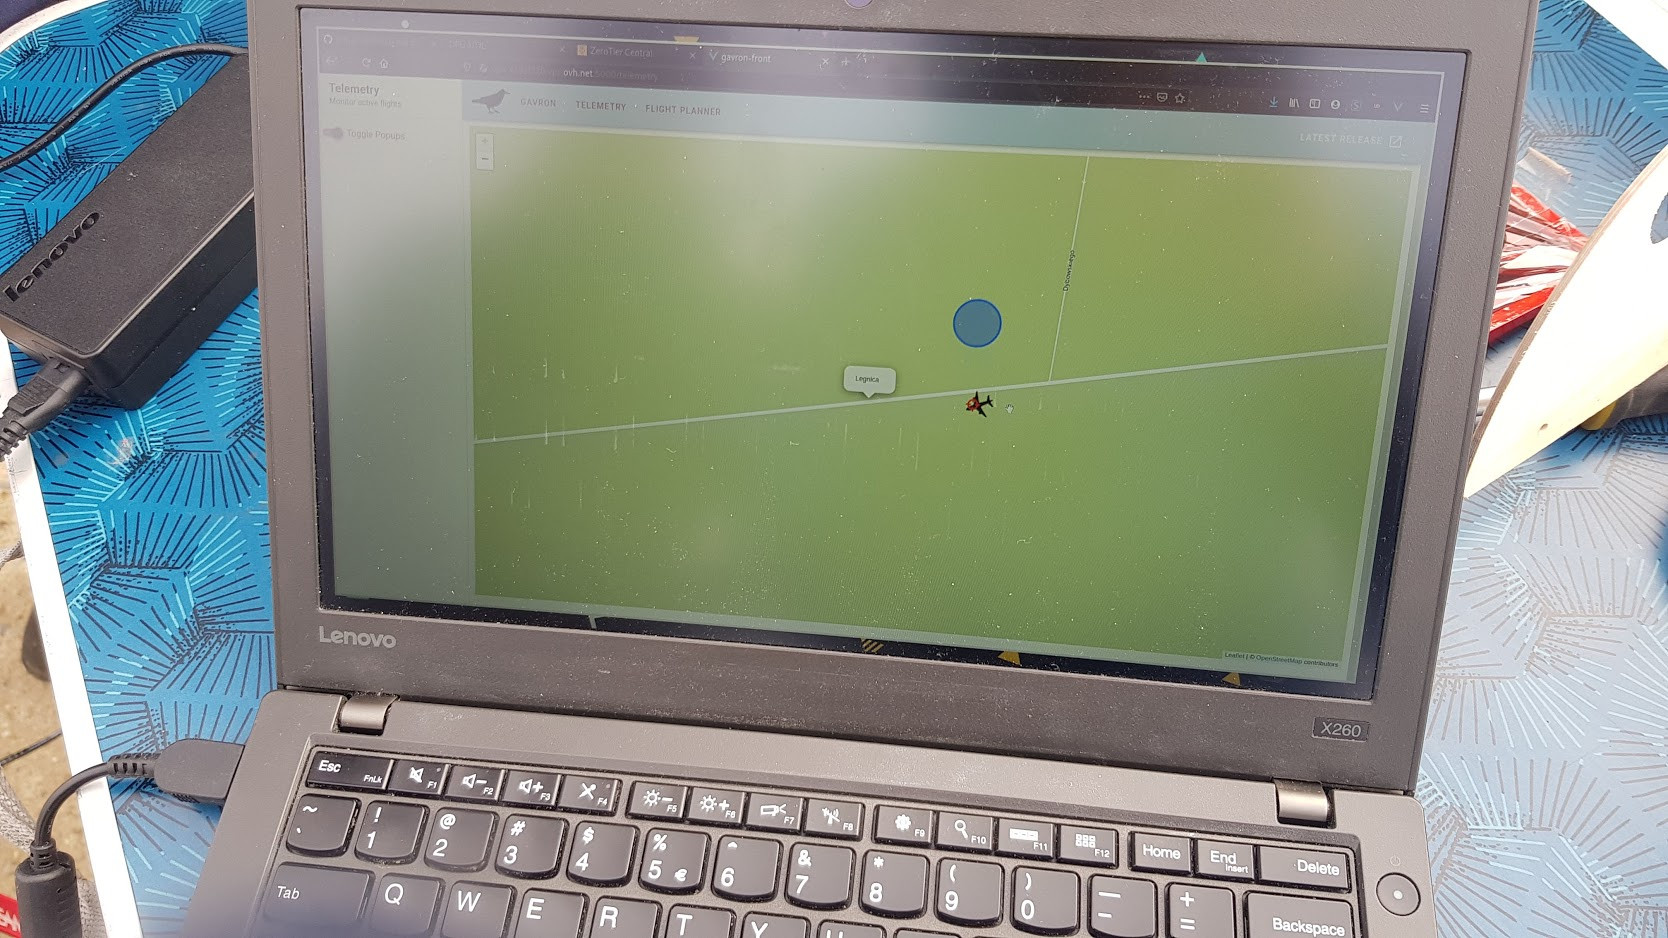
\includegraphics[width=0.8\linewidth]{rys05/sae_telem.jpg}
    \caption{
        Wczesna wersja aplikacji klienckiej, wyświetlająca pozycję samolotu w trakcie lotu.
    }
	\label{telem_sae}
\end{figure}

Jak wspomniano w podrozdziale \ref{ouroboros}, automatyczne aktualizowanie infrastruktury
internetowej systemu pozwoliło na szybsze i bezpieczniejsze wprowadzanie poprawek w systemie.
Jest to szczególnie pożądane w przypadku testowania dronów/samolotów, ponieważ przeprowadzenie
lotu wymaga obecności całego zespołu: mechaników, elektroników, programistów oraz pilota. Szybsze
wprowadzanie zmian w oprogramowaniu umożliwia sprawniejsze wykonywanie lotów i wykonanie
większej ilości lotów testowych.

\subsection{Finalne testy systemu}
\subsection{Platforma testowa}
\begin{figure}[H]
	\centering
	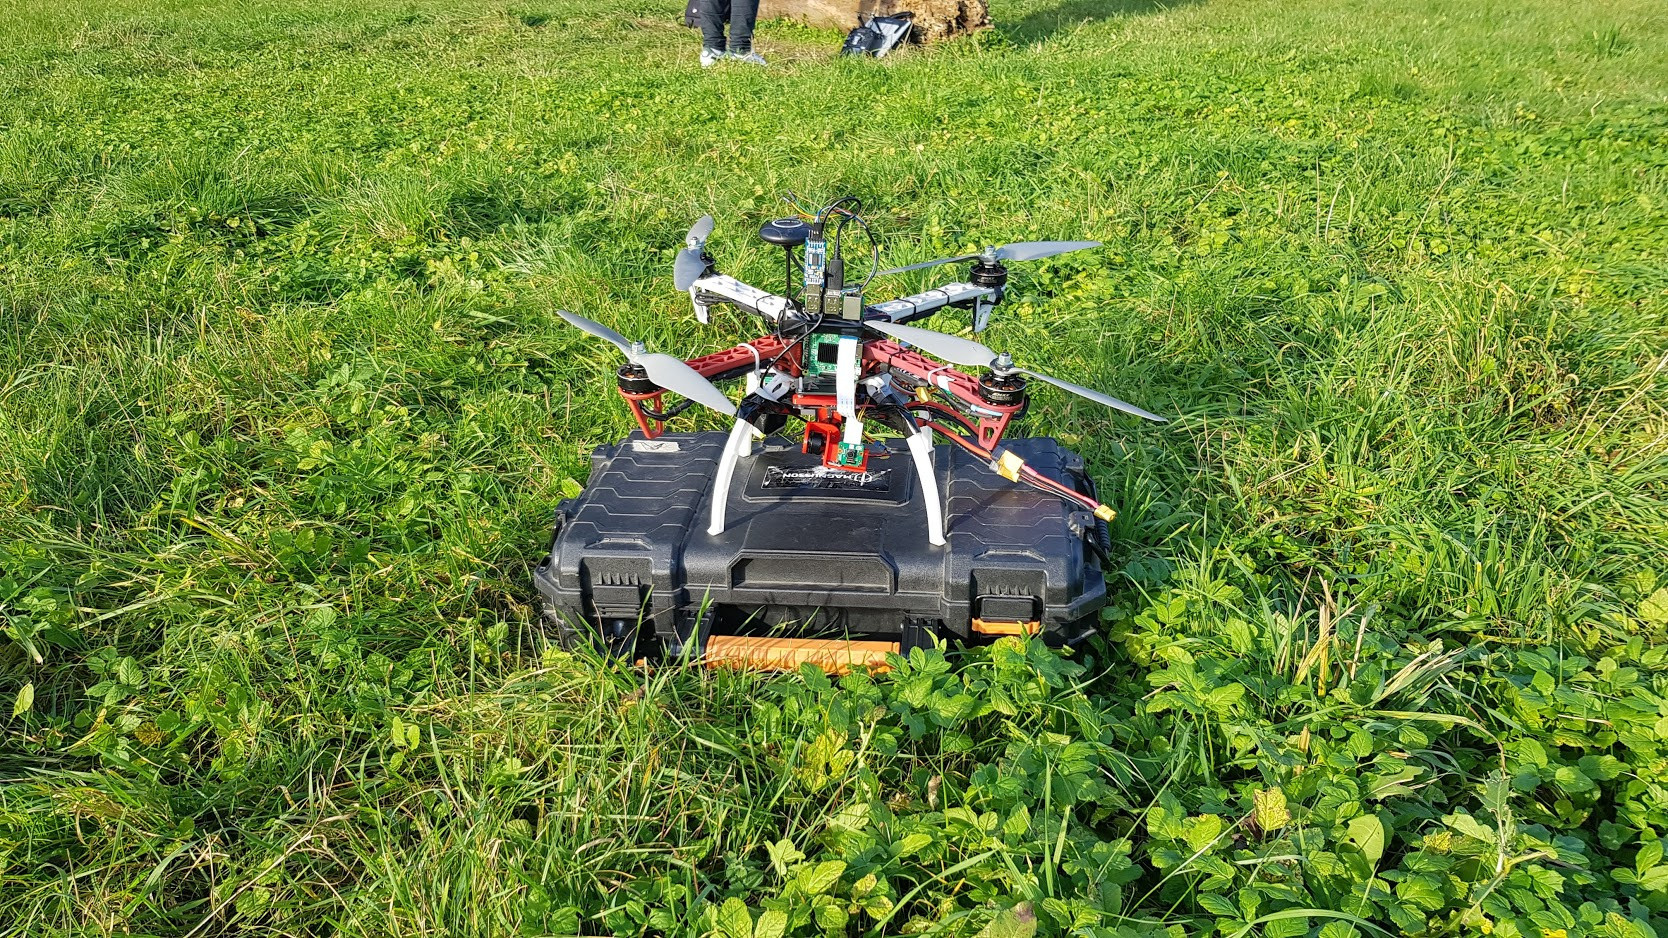
\includegraphics[width=0.8\linewidth]{rys05/testing_drone.jpg}
    \caption{
        Dron wykorzystywany do finałowych testów projektu.
    }
	\label{testing_drone}
\end{figure}


Finalnie wykorzystywany dron, przedstawiony na rysunku \ref{testing_drone}, zawierał
ten sam kontroler lotu co samolot używany do wczesnych testów, opisanych w podrozdziale 
\ref{early_tests}. Dodatkowo, dron zaopatrzony był w kamerę na gimbalu.

\subsection{Przebieg lotów testowych}

W trakcie lotów testowych kilkakrotnie został wykonany scenariusz 
wykorzystania systemu, opisany w celu pracy (\ref{intro_objective}):

\begin{enumerate}
    \item W aplikacji klienckiej wyznaczona została nowa trasa lotu,
    \item dron pobrał trasę i rozkład lotu z serwera \textit{REST API},
    \item dron wystartował, po czym zaczął wysyłać dane telemetryczne i zdjęcia (\ref{final_frontend}),
    \item dane telemetryczne i wykonane zdjęcia zostały przekazane do aplikacji klienckiej,
    \item odebrane na serwerze zdjęcia zostały przetworzone przez algorytmy sztucznej inteligencji,
        które rozpoznały obecnych na zdjęciach ludzi (\ref{final_ai_good}).
\end{enumerate}

\begin{figure}[H]
	\centering
	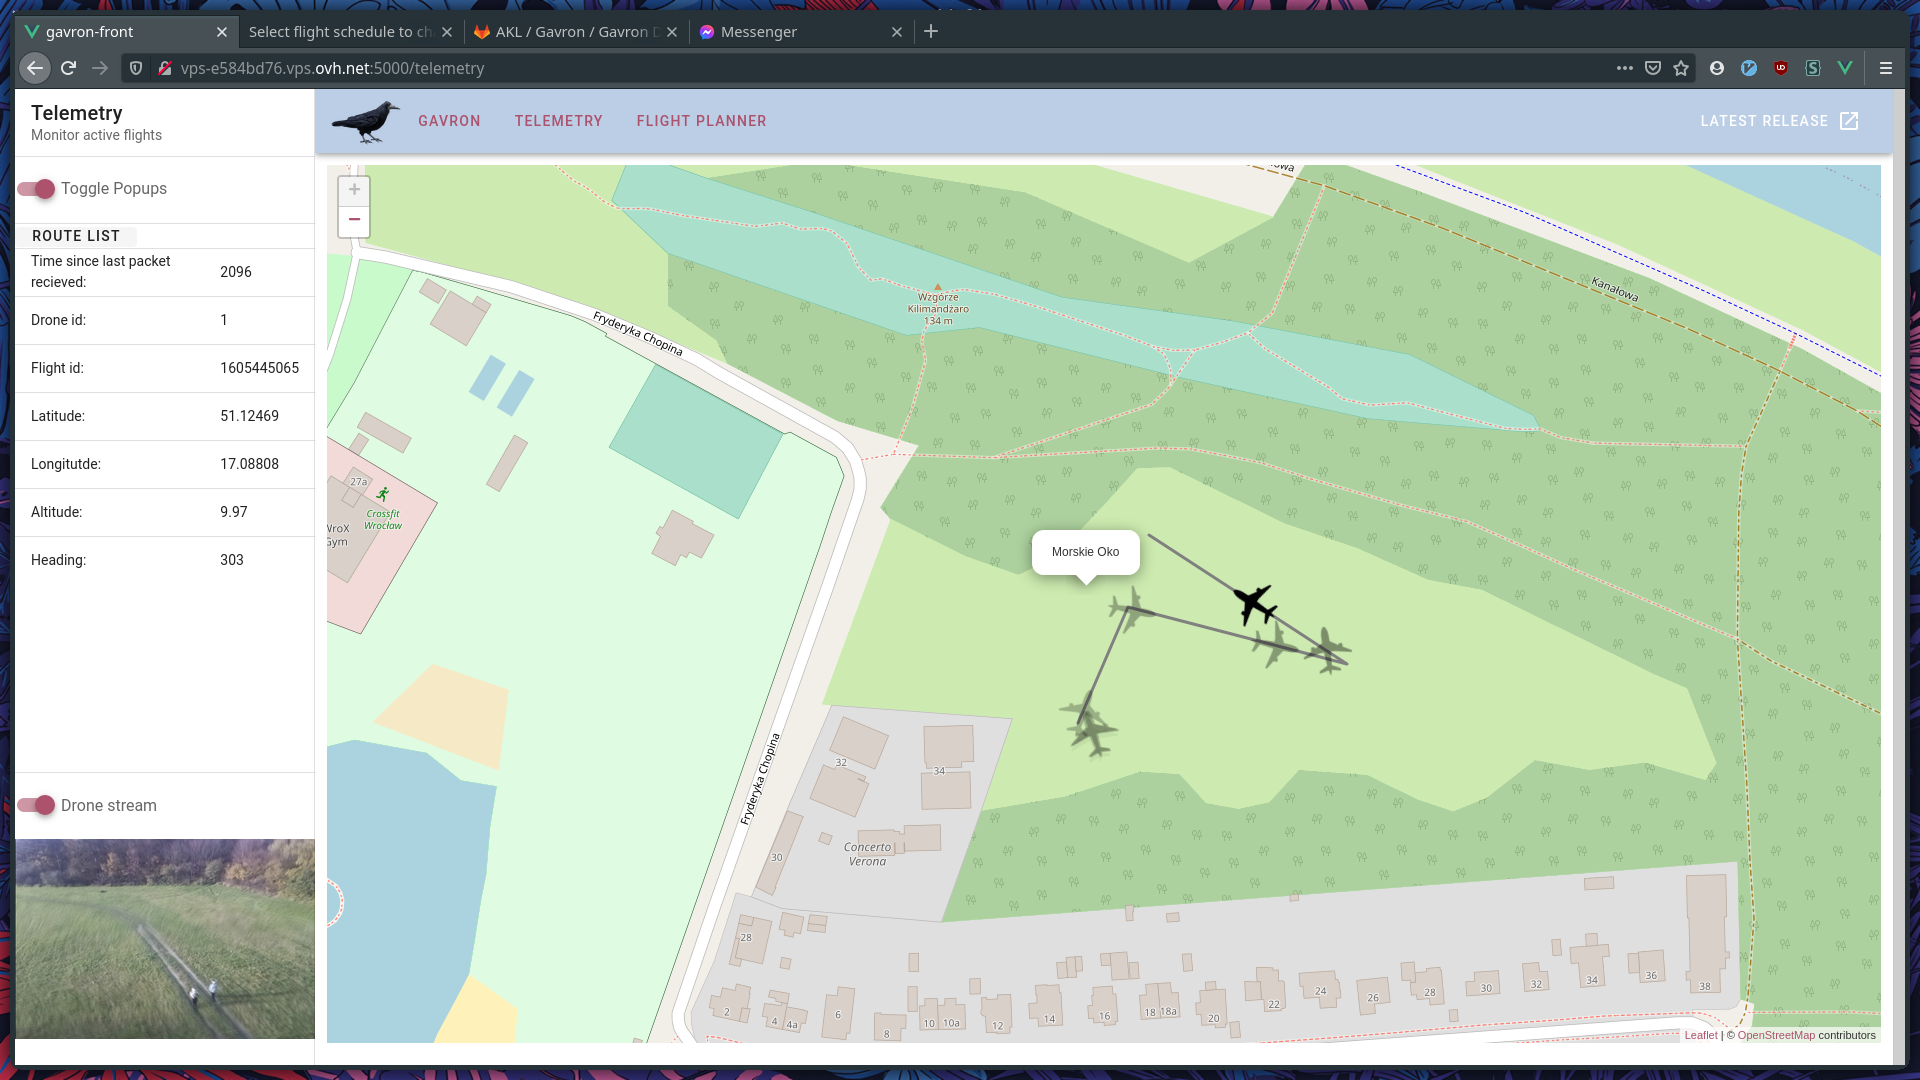
\includegraphics[width=0.8\linewidth]{rys05/final_flight_telem.png}
    \caption{
        Finalna wersja aplikacji klienckiej w trakcie testów w terenie. 
        W prawym dolnym rogu widoczny podgląd zdjęć wykonywanych w trakcie lotu,
        przesyłanych w czasie rzeczywistym do aplikacji.
    }
	\label{final_frontend}
\end{figure}

Aplikacja kliencka, widoczna na rysunku \ref{final_frontend} wyświetla zaplanowaną
wcześniej trasę przelotu oraz pozycję drona, odczytaną z danych telemetrycznych.
Pozycja maszyny jest aktualizowana w czasie rzeczywistym. Równolegle odbierane
są nowe zdjęcia wykonane w czasie lotu.

\subsection{Rozpoznawanie obiektów na zdjęciach}
\begin{multicols}{2}
    
\begin{figure}[H]
	\centering
	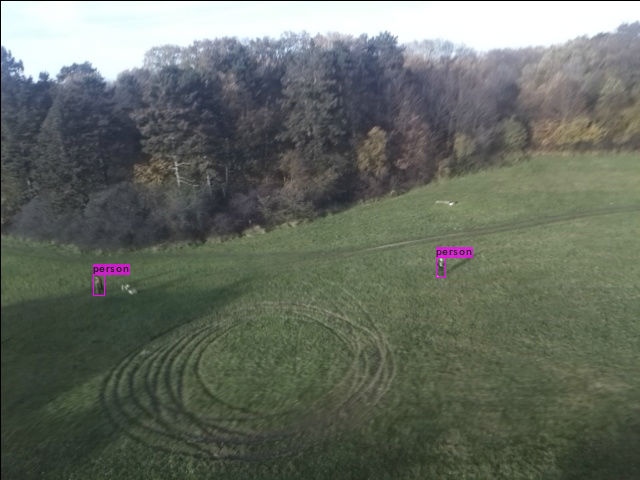
\includegraphics[width=\linewidth]{rys05/correctly_recognised_2_ppl.jpg}
    \caption{
        Zdjęcie wykonane podczas lotu, na zdjęciu poprawnie rozpoznano dwie osoby.
    }
	\label{final_ai_good}
\end{figure}

\begin{figure}[H]
	\centering
	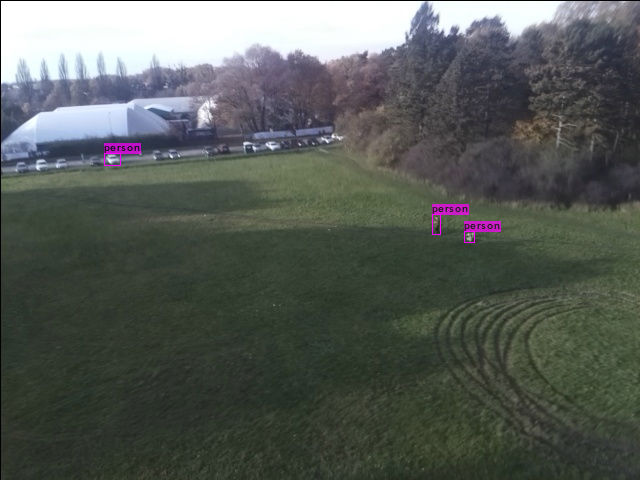
\includegraphics[width=\linewidth]{rys05/car_person.jpg}
    \caption{
        Zdjęcie wykonane podczas lotu. Samochód został niepoprawnie oznaczony jako osoba.
    }
	\label{final_ai_bad}
\end{figure}
\end{multicols}

Algorytmy sztucznej inteligencji, omówione w podrozdziale \ref{yolo} 
próbowały rozpoznać ludzi na zdjęciach wykonanych w trakcie lotów.
Większość zdjęć została rozpoznana poprawnie, system nie rozpoznawał
głównie zdjęć, które były niewyraźne. Rysunki \ref{final_ai_good} i \ref{final_ai_bad}
zawierają przykładowe zdjęcia wraz z oznaczonymi na obiektami.
Diagram \ref{ai_results} zawiera podsumowanie dokładności rozpoznawania
ludzi, obliczonej na podstawie wszystkich zdjęć wykonanych podczas lotów.

\begin{figure}[H]
	\centering
    \begin{tikzpicture}[align=center]
        
        \pie [
            rotate = 0,
            /tikz/every pin/.style={align=center},
            explode=0.2,
            color={green!50,orange!70,red!70}
            ]
        {
            76/Ludzie poprawnie\\ rozpoznani,
            9/Ludzie nierozpoznani{,}\\nie w pełni widoczni na zdjęciu,
            15/Ludzie nierozpoznani{,}\\ mimo że byli w pełni\\ widoczni na zdjęciu
        }
    \end{tikzpicture}

    \caption{
        Dokładność z jaką rozpoznawani są ludzie na zdjęciach wykonanych podczas lotów
    }
	\label{ai_results}
\end{figure}

% 31 na zdjęciach
% 26 rozpoznanych
% 3 osoby ucięte w połowie, ciężko powiedzieć
% 1 raz samochód rozpoznany jako osoba

